\chapter{Arrangements of Lines and Curves}
\label{ch:envelopes}

\section{Davenport--Schinzel Sequences}
\label{sec:davenport_schinzel}

\subsection{Overview}
A Davenport--Schinzel sequence\index{Davenport--Schinzel sequence} is a sequence of symbols that satisfies specific constraints on the alternating sub-sequences it can contain. These sequences provide a powerful combinatorial framework for analyzing the complexity of the \textbf{lower envelope} of a set of functions. In computational geometry, they are used to bound the complexity of arrangements of curves, motion planning visibility, and dynamic geometric structures. The theory originated with Davenport and Schinzel~\cite{davenport1965} and was developed into a comprehensive geometric theory by Sharir and Agarwal~\cite{sharir1995}.

\subsection{Definitions}

\begin{definition}[Davenport--Schinzel Sequence]\label{def:ds_sequence}
A sequence $U = (u_1, u_2, \dots, u_m)$ over an alphabet $A$ of $n$ symbols is a \textbf{Davenport--Schinzel sequence of order $s$}\index{Davenport--Schinzel sequence} (denoted $\text{DS}(n,s)$) if:
\begin{enumerate}
    \item No two adjacent symbols are the same: $u_i \neq u_{i+1}$ for all $1 \leq i < m$.
    \item It does not contain any alternating sub-sequence of length $s+2$ of the form $a, b, a, b, \dots$ (alternating $s+1$ times between two distinct symbols $a, b \in A$).
\end{enumerate}
\end{definition}

\begin{definition}[$\lambda_s(n)$]\label{def:lambda_s}
$\lambda_s(n)$\index{$\lambda_s(n)$} denotes the maximum possible length of a Davenport--Schinzel sequence of order $s$ on $n$ distinct symbols. These functions grow near-linearly for any fixed $s$:
\[
\lambda_0(n) = 1, \quad \lambda_1(n) = n, \quad \lambda_2(n) = 2n - 1, \quad \lambda_3(n) = \Theta(n\,\alpha(n)),
\]
where $\alpha(n)$ is the inverse Ackermann function.
\end{definition}

\begin{definition}[Inverse Ackermann Function]\label{def:inverse_ackermann}
The \textbf{inverse Ackermann function}\index{inverse Ackermann function} $\alpha(n)$ is the function such that $\alpha(n) \leq 4$ for all practical values of $n$ (up to $n = 10^{80}$, the number of atoms in the observable universe). Formally, $\alpha(n)$ is the inverse of the Ackermann function $A(k)$, which grows faster than any primitive recursive function.
\end{definition}

\begin{definition}[Lower Envelope]\label{def:lower_envelope_ds}
The \textbf{lower envelope}\index{lower envelope} of a collection of $n$ functions $\{f_1, \dots, f_n\}$ defined on a common domain $D$ is the function $L(x) = \min_{1 \leq i \leq n} f_i(x)$. The \emph{complexity} of the lower envelope is the number of maximal continuous pieces that compose it.
\end{definition}

\subsection{Theory}

The importance of DS sequences stems from their relationship to function intersections. If we have $n$ continuous functions such that any two functions intersect at most $s$ times, then the sequence of function indices that form the \textbf{lower envelope} is a Davenport--Schinzel sequence of order~$s$.

For example:
\begin{itemize}
    \item \textbf{Order $s=1$}: Functions intersect at most once (e.g., lines). $\lambda_1(n) = n$.
    \item \textbf{Order $s=2$}: Functions intersect at most twice (e.g., parabolas). $\lambda_2(n) = 2n - 1$.
    \item \textbf{Order $s=3$}: Functions intersect at most three times. $\lambda_3(n) = \Theta(n \alpha(n))$, where $\alpha(n)$ is the extremely slow-growing inverse Ackermann function.
\end{itemize}

This theory allows us to prove that the complexity of the lower envelope of $n$ line segments is $O(n \alpha(n))$, which is much smaller than the total number of intersections $O(n^2)$.

\begin{theorem}[DS Sequence Length Bounds]\label{thm:ds_bounds}
For $s \geq 1$ and $n \geq 1$:
\begin{enumerate}
    \item $\lambda_1(n) = n$.
    \item $\lambda_2(n) = 2n - 1$.
    \item For $s \geq 3$, $\lambda_s(n) = n \cdot \alpha(n)^{O(1)}$, where $\alpha(n)$ is the inverse Ackermann function. More precisely, $\lambda_3(n) = 2n\alpha(n) + O(n)$.
\end{enumerate}
These bounds are tight.
\end{theorem}

\begin{proof}
The cases $s = 1$ and $s = 2$ are elementary. For $s \geq 3$, the upper bound was established by Sharir~\cite{sharir1995} using a charging argument on the ``blocks'' of the sequence and the properties of the Ackermann hierarchy. The matching lower bound is obtained by an explicit construction based on the composition sequences of the Ackermann function. See~\cite[Chapters~2--4]{sharir1995} for the complete proof.
\end{proof}

\begin{observation}
The growth rate of $\lambda_s(n)$ for increasing $s$ reflects the increasing complexity of the lower envelope as the number of allowed intersections between function pairs grows. For $s = 1$ (lines), the envelope has $O(n)$ complexity. For $s = 3$ (line segments), the complexity jumps to $O(n \alpha(n))$---a subtlety that arises from the non-monotonic behavior of segments.
\end{observation}

\subsection{Pseudocode}

\subsubsection*{Computing the Lower Envelope (Recursive)}
\begin{algorithm}[ht]
\label{alg:lower_envelope_recursive}
\begin{algorithmic}[1]
\Function{LowerEnvelope}{$\text{functions}$, $\text{start}$, $\text{end}$}
    \If{$|\text{functions}| = 1$}
        \State \Return $\text{functions}[0]$
    \EndIf
    \State $\text{mid} \gets |\text{functions}| / 2$
    \State $\text{left\_env} \gets \text{LowerEnvelope}(\text{functions}[:\text{mid}],\; \text{start},\; \text{end})$
    \State $\text{right\_env} \gets \text{LowerEnvelope}(\text{functions}[\text{mid}:],\; \text{start},\; \text{end})$
    \State $\text{merged\_env} \gets \text{MergeEnvelopes}(\text{left\_env},\; \text{right\_env})$
    \State \Return $\text{merged\_env}$
\EndFunction

\Function{MergeEnvelopes}{$E1$, $E2$}
    \State $\text{intersections} \gets \text{FindIntersections}(E1,\; E2)$
    \State \Return $\text{ResultingSequence}(E1,\; E2,\; \text{intersections})$
\EndFunction
\end{algorithmic}
\end{algorithm}

\subsection{Parameter Selection}
\begin{itemize}
    \item \textbf{Order ($s$)}: Depends on the type of geometric primitives (e.g., $s=1$ for lines, $s=2$ for circles, $s=3$ for line segments).
    \item \textbf{Alphabet Size ($n$)}: The number of geometric objects.
\end{itemize}

\subsection{Complexity}
\begin{itemize}
    \item \textbf{Maximum Length}: $\lambda_s(n)$ is near-linear for any fixed $s$. For example, $\lambda_3(n) = O(n \alpha(n))$.
    \item \textbf{Construction Time}: The lower envelope can be computed in $O(\lambda_s(n) \log n)$ time using a divide-and-conquer approach.
\end{itemize}

\subsection{Usages}
\begin{itemize}
    \item \textbf{Arrangements}\index{arrangements}: Bounding the number of edges on a single cell or the lower envelope of an arrangement of curves.
    \item \textbf{Motion Planning}: Analyzing the complexity of the ``free space'' for a robot moving among obstacles.
    \item \textbf{Visibility}: Calculating the complexity of the region visible from a point in a dynamic environment.
    \item \textbf{Kinetic Data Structures}\index{kinetic data structure}: Tracking the minimum value among a set of moving points.
    \item \textbf{Shortest Paths}: Computing the visibility graph of a set of segments.
\end{itemize}

\subsection{Testing Methods and Edge Cases}
\begin{itemize}
    \item \textbf{Non-Intersecting Functions}: The envelope should simply follow the lowest function for the entire range.
    \item \textbf{Multiple Intersections}: Ensure the algorithm correctly captures all points where the lower envelope switches from one function to another.
    \item \textbf{Touching vs.\ Crossing}: Handle cases where functions are tangent to each other without crossing.
    \item \textbf{Vertical Segments}: Ensure the interval logic handles vertical discontinuities.
    \item \textbf{Complexity Check}: Verify that the number of segments in the resulting envelope is within the DS bound $\lambda_s(n)$.
\end{itemize}

\subsection{References}
\begin{itemize}
    \item Davenport, H., \& Schinzel, A. (1965). ``A combinatorial problem connected with differential equations''. American Journal of Mathematics.
    \item Sharir, M., \& Agarwal, P.~K. (1995). ``Davenport--Schinzel Sequences and Their Geometric Applications''. Cambridge University Press.
    \item Atallah, M.~J. (1985). ``Some dynamic computational geometry problems''. Computers \& Mathematics with Applications.
    \item Wikipedia: \href{https://en.wikipedia.org/wiki/Davenport\%E2\%80\%93Schinzel_sequence}{Davenport--Schinzel sequence}
\end{itemize}

\section{Lower Envelopes}
\label{sec:lower_envelopes}

\subsection{Overview}
The lower envelope\index{lower envelope} of a set of functions $f_1, f_2, \dots, f_n$ is the pointwise minimum of those functions: $L(x) = \min_i f_i(x)$. In computational geometry, the lower envelope is a fundamental structure used to solve problems related to visibility, optimization, and arrangements. For example, the lower envelope of a set of lines forms the boundary of their intersection (a convex polygon in the dual plane). The computational aspects of envelopes were studied extensively by Edelsbrunner~\cite{edelsbrunner1987} and Hershberger~\cite{hershberger1989}.

\subsection{Definitions}

\begin{definition}[Lower Envelope]\label{def:lower_envelope}
The \textbf{lower envelope}\index{lower envelope} of a family of functions $\{f_1, \dots, f_n\}$ on a domain $D \subseteq \mathbb{R}$ is the function $L: D \to \mathbb{R}$ defined by $L(x) = \min_{1 \leq i \leq n} f_i(x)$. The envelope is piecewise composed of segments of the individual functions.
\end{definition}

\begin{definition}[Upper Envelope]\label{def:upper_envelope}
The \textbf{upper envelope}\index{upper envelope} of a family of functions $\{f_1, \dots, f_n\}$ is $U(x) = \max_{1 \leq i \leq n} f_i(x)$. The upper envelope of a set of functions is the lower envelope of their negations.
\end{definition}

\begin{definition}[Minimization Diagram]\label{def:minimization_diagram}
A \textbf{minimization diagram}\index{minimization diagram} is the partition of the domain $D$ into maximal regions where a specific function $f_i$ achieves the minimum. Each region is called a \emph{cell} of the diagram, and the boundary between two cells is formed by the intersection points of the corresponding functions.
\end{definition}

\begin{definition}[Complexity of an Envelope]\label{def:envelope_complexity}
The \textbf{complexity}\index{envelope complexity} of a lower envelope is the number of maximal continuous pieces (arcs) that compose it. Each arc is a maximal connected subset of the domain on which a single function $f_i$ achieves the pointwise minimum.
\end{definition}

\subsection{Theory}
The complexity of the lower envelope depends on how many times any two functions can intersect.
\begin{enumerate}
    \item \textbf{Lines}: Any two lines intersect at most once. The lower envelope of $n$ lines is a convex chain with at most $n$ segments.
    \item \textbf{Line Segments}: Two segments can intersect at most once, but the envelope can have up to $O(n \alpha(n))$ segments due to the ``visibility'' of segments behind each other.
    \item \textbf{Parabolas/Circles}: Two functions intersect at most twice. The envelope complexity is $O(n)$.
    \item \textbf{General Curves}: If any two curves intersect at most $s$ times, the complexity is bounded by the Davenport--Schinzel sequence $\lambda_s(n)$.
\end{enumerate}

The lower envelope can be computed using a \textbf{Divide and Conquer} algorithm\index{divide and conquer}:
\begin{enumerate}
    \item Divide the set of functions into two halves.
    \item Recursively compute the lower envelope of each half.
    \item Merge the two envelopes by finding their intersection points and keeping the lower segments.
\end{enumerate}

\begin{theorem}[Lower Envelope Complexity for Lines]\label{thm:lower_envelope_lines}
The lower envelope of $n$ lines in $\mathbb{R}^2$ consists of at most $n$ segments and can be computed in $O(n \log n)$ time.
\end{theorem}

\begin{proof}
Any two distinct lines intersect in at most one point. By the DS sequence framework with $s = 1$, the envelope is a $\text{DS}(n, 1)$ sequence, which has length at most $n$. The divide-and-conquer algorithm solves the recurrence $T(n) = 2T(n/2) + O(n)$, giving $T(n) = O(n \log n)$.
\end{proof}

\begin{theorem}[Lower Envelope Complexity for Segments]\label{thm:lower_envelope_segments}
The lower envelope of $n$ line segments in $\mathbb{R}^2$ has $O(n\,\alpha(n))$ complexity, where $\alpha(n)$ is the inverse Ackermann function, and can be computed in $O(n\,\alpha(n) \log n)$ time.
\end{theorem}

\begin{proof}
Any two line segments intersect in at most one point (since they are linear), so the envelope is a DS sequence of order $s = 3$ (segments can cross, touch, or miss). The DS bound $\lambda_3(n) = O(n\,\alpha(n))$ gives the complexity upper bound. The divide-and-conquer algorithm merges two sub-envelopes in time proportional to their combined complexity times $\log n$, yielding $O(n\,\alpha(n) \log n)$ total time. See Edelsbrunner~\cite[Chapter~4]{edelsbrunner1987}.
\end{proof}

\begin{figure}[htbp]
\centering
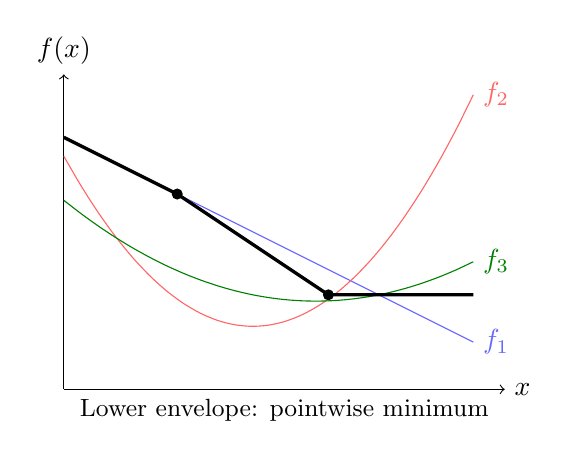
\begin{tikzpicture}[scale=0.8]
  \draw[->] (0,0)--(7,0) node[right] {$x$};
  \draw[->] (0,0)--(0,5) node[above] {$f(x)$};
  \draw[blue!60,domain=0:6.5,smooth] plot (\x,{4-0.5*\x}) node[right,blue!60] {$f_1$};
  \draw[red!60,domain=0:6.5,smooth] plot (\x,{1+0.3*(\x-3)^2}) node[right,red!60] {$f_2$};
  \draw[green!50!black,domain=0:6.5,smooth] plot (\x,{3-0.8*\x+0.1*\x*\x}) node[right,green!50!black] {$f_3$};
  \draw[very thick,black] (0,4) -- (1.8,3.1) -- (4.2,1.5) -- (6.5,1.5);
  \fill (1.8,3.1) circle (2.5pt);
  \fill (4.2,1.5) circle (2.5pt);
  \node[below,font=\small] at (3.5,0) {Lower envelope: pointwise minimum};
\end{tikzpicture}
\caption{Lower envelope of three functions: the thick black curve is the pointwise minimum $\min\{f_1, f_2, f_3\}$.}
\label{fig:lower_envelope}
\end{figure}


\begin{example}[Lower Envelope of Lines]\label{ex:lower_envelope_lines}
Consider four lines: $f_1(x) = 2 - x$, $f_2(x) = -1 + 2x$, $f_3(x) = 3 - 0.5x$, $f_4(x) = x - 2$.
The lower envelope is:
\[
L(x) = \min(2 - x,\; -1 + 2x,\; 3 - 0.5x,\; x - 2)
\]
On $(-\infty, 0)$: $f_4(x) = x-2$ is the minimum. On $[0, 1]$: $f_1(x) = 2-x$ is minimum. On $[1, 2]$: $f_2(x) = -1+2x$ is minimum. On $(2, \infty)$: $f_4(x) = x-2$ is minimum again. The envelope has 4 pieces, which does not exceed $n = 4$.
\end{example}

\subsection{Pseudocode}
\begin{algorithm}[ht]
\label{alg:compute_lower_envelope}
\begin{algorithmic}[1]
\Function{ComputeLowerEnvelope}{$\text{functions}$, $x_{\min}$, $x_{\max}$}
    \If{$|\text{functions}| = 1$}
        \State \Return $[(\text{functions}[0],\; x_{\min},\; x_{\max})]$
    \EndIf
    \State $\text{mid} \gets |\text{functions}| / 2$
    \State $\text{left\_env} \gets \text{ComputeLowerEnvelope}(\text{functions}[:\text{mid}],\; x_{\min},\; x_{\max})$
    \State $\text{right\_env} \gets \text{ComputeLowerEnvelope}(\text{functions}[\text{mid}:],\; x_{\min},\; x_{\max})$
    \State $\text{merged} \gets []$
    \For{$\text{segment\_L}$ in $\text{left\_env}$}
        \For{$\text{segment\_R}$ in $\text{right\_env}$}
            \State $\text{common\_start} \gets \max(\text{segment\_L}.\text{start},\; \text{segment\_R}.\text{start})$
            \State $\text{common\_end} \gets \min(\text{segment\_L}.\text{end},\; \text{segment\_R}.\text{end})$
            \If{$\text{common\_start} < \text{common\_end}$}
                \State $\text{intersections} \gets \text{FindIntersections}(\text{segment\_L}.f,\; \text{segment\_R}.f,\; \text{common\_start},\; \text{common\_end})$
                \State $\text{merged}.\text{extend}(\text{PickLower}(\text{segment\_L}.f,\; \text{segment\_R}.f,\; \text{common\_start},\; \text{common\_end},\; \text{intersections}))$
            \EndIf
        \EndFor
    \EndFor
    \State \Return $\text{Simplify}(\text{merged})$
\EndFunction
\end{algorithmic}
\end{algorithm}

\subsection{Parameter Selection}
\begin{itemize}
    \item \textbf{Function Type}: Linear, polynomial, or arbitrary continuous functions.
    \item \textbf{Intersection Solver}: A robust numerical or symbolic solver is needed to find where $f_i(x) = f_j(x)$.
\end{itemize}

\subsection{Complexity}
\begin{itemize}
    \item \textbf{Complexity of Envelope}: $O(\lambda_s(n))$ where $s$ is the number of intersections.
    \item \textbf{Construction Time}: $O(\lambda_s(n) \log n)$ using divide and conquer.
    \item \textbf{Space Complexity}: $O(\lambda_s(n))$ to store the resulting segments.
\end{itemize}

\subsection{Usages}
\begin{itemize}
    \item \textbf{Visibility}: Calculating the ``horizon'' of a set of mountains or the region visible from a point.
    \item \textbf{Motion Planning}: Finding the safest path by maximizing the distance to the nearest obstacle (lower envelope of distance functions).
    \item \textbf{Duality}: Solving problems like the ``Width of a Point Set'' or ``Diameter'' in the dual plane.
    \item \textbf{Dynamic Programming}: Optimizing decisions over time where costs are modeled as functions.
    \item \textbf{Statistics}: Calculating the ``support'' of a probability distribution.
\end{itemize}

\subsection{Testing Methods and Edge Cases}
\begin{itemize}
    \item \textbf{Non-Intersecting Functions}: The envelope should simply be the single function that is globally minimum.
    \item \textbf{Vertical Functions}: Ensure the algorithm handles discontinuities or vertical lines.
    \item \textbf{Touching Functions}: Verify that tangencies (where functions touch but don't cross) don't create unnecessary segments.
    \item \textbf{Overlap}: Handle cases where two functions are identical over an interval.
    \item \textbf{Large $n$}: Verify the near-linear growth of the result size.
\end{itemize}

\subsection{References}
\begin{itemize}
    \item Sharir, M., \& Agarwal, P.~K. (1995). ``Davenport--Schinzel Sequences and Their Geometric Applications''. Cambridge University Press.
    \item Hershberger, J. (1989). ``Finding the upper envelope of $n$ line segments in $O(n \log n)$ time''. Information Processing Letters.
    \item Edelsbrunner, H. (1987). ``Algorithms in Combinatorial Geometry''. Springer-Verlag.
    \item Wikipedia: \href{https://en.wikipedia.org/wiki/Lower_envelope}{Lower envelope}
\end{itemize}

\section{Levels in Arrangements and Half-Plane Discrepancy}
\label{sec:arrangement_levels}

\subsection{Overview}
In an arrangement of lines, every point not on a line has a well-defined
\emph{level}: the number of lines strictly below it. The set of points of a
fixed level is a polygonal chain called the \textbf{k-level}\index{k-level},
which generalizes the lower envelope (level $0$) and the upper envelope (level
$n-1$). Levels are the bridge between arrangements and point sets: by duality,
the vertices of the $k$-level of an arrangement of lines correspond exactly to
the \textbf{k-sets} of the dual point set---subsets of size $k$ separable from
the rest by a line. Levels also control the \textbf{half-plane
discrepancy}\index{half-plane discrepancy} of a point set, a measure of how
well a set of $n$ points approximates the uniform distribution that arises,
for example, in the supersampling analysis of ray tracing~\cite{sharir1995}.

\subsection{Definitions}

\begin{definition}[Level of a Point]\label{def:point_level}
In an arrangement $\mathcal{A}(\mathcal{L})$ of $n$ lines, the \emph{level} of
a point $p$ that lies on no line is the number of lines of $\mathcal{L}$
strictly below $p$. The \emph{$k$-level} is the set of points whose level is
exactly $k$; it is an $x$-monotone polygonal chain. The \emph{complexity} of
the $k$-level is its number of vertices.
\end{definition}

\begin{definition}[k-Set]\label{def:kset}
A \emph{$k$-set} of a point set $P$ is a subset $K \subseteq P$ with $|K| = k$
that can be separated from $P \setminus K$ by a line. Under point--line
duality, the $k$-sets of $P$ correspond one-to-one with the vertices of the
$k$-th level of the arrangement of lines dual to $P$.
\end{definition}

\begin{definition}[Half-Plane Discrepancy]\label{def:halfplane_discrepancy}
Let $P$ be a set of $n$ points inside a region $B$ of area $1$. The
\emph{half-plane discrepancy} of $P$ is
\[
D(P) = \max_{h \text{ half-plane}} \bigl|\, |P \cap h| - n \cdot \operatorname{area}(h \cap B) \,\bigr|.
\]
The discrepancy $D(n)$ is the minimum of $D(P)$ over all $n$-point sets $P$.
\end{definition}

\subsection{Theory}

The lower envelope studied in Section~\ref{sec:lower_envelopes} is precisely
the $0$-level, and the upper envelope is the $(n-1)$-level. The complexity of
intermediate levels is the central open problem of the area; the best known
results are as follows.

\begin{theorem}[Complexity of the k-Level]\label{thm:level_complexity}
The complexity of the $k$-th level in an arrangement of $n$ lines is
$O(n k^{1/3})$ for every $k$~\cite{dey1998}; for the middle level ($k \approx
n/2$) this is $O(n^{4/3})$. The best known lower bound is
$n\,2^{\Omega(\sqrt{\log k})}$.
\end{theorem}
\begin{proof}[Proof sketch]
The older bound $O(n \sqrt{k})$ of Lov\'asz follows by a potential-function
argument: sweep the arrangement and charge the $\Omega(\sqrt{k})$ left-turning
vertices of the level. Dey's improvement applies the crossing lemma to the
union of $k$ x-monotone concave chains that cover the region below the level,
yielding the $O(nk^{1/3})$ bound~\cite{dey1998}.
\end{proof}

The connection between levels and discrepancy is that a half-plane whose
incidence count deviates strongly from the area expectation must contain many
vertices of a level in the dual arrangement; hence a low-discrepancy point set
forces every level to be simple.

\begin{theorem}[Half-Plane Discrepancy of n Points]\label{thm:halfplane_discrepancy}
The half-plane discrepancy of every set of $n$ points is at least
$c\,n^{1/4}$, and there exist $n$-point sets (such as suitable lattices) whose
half-plane discrepancy is $O(n^{1/4})$. In particular $D(n) = \Theta(n^{1/4})$.
\end{theorem}
\begin{proof}[Proof sketch]
The lower bound is due to Beck and Alexander using Fourier-analytic
(integral-geometric) techniques~\cite{matousek1999}. The matching upper bound
is due to Matou\v{s}ek, who constructed point sets---related to scaled integer
lattices---for which every half-plane counts the expected number of points up
to an error of $O(n^{1/4})$~\cite{matousek1995,matousek1999}.
\end{proof}

\subsection{Pseudocode}

A simple incremental construction of the $k$-level of an arrangement of $n$
lines uses the duality between levels and k-sets.

\begin{algorithm}[ht]
\label{alg:compute_klevel}
\caption{Compute the k-Level of a Line Arrangement}
\begin{algorithmic}[1]
\Function{ComputeKLevel}{lines, k}
  \State $\mathcal{A} \gets \text{LineArrangement}(lines)$
  \State $\text{level} \gets 0$
  \State $p \gets$ point at $x = -\infty$ on the lowest line of $\mathcal{A}$
  \While{$x \ne +\infty$}
    \If{$\text{level} = k$}
      \State append the current edge to the output chain
    \EndIf
    \State advance to the next vertex of $\mathcal{A}$
    \State $\text{level} \gets \text{level} \pm 1$ \Comment{crossing a line}
  \EndWhile
  \State \Return the output chain
\EndFunction
\end{algorithmic}
\end{algorithm}

\subsection{Parameter Selection}
\begin{itemize}
    \item \textbf{Level $k$}: choose $k = 0$ for the lower envelope and
      $k = n - 1$ for the upper envelope; intermediate $k$ give the $k$-sets.
    \item \textbf{Duality}: for discrepancy problems, dualize the point set to
      lines and operate on levels of the arrangement.
\end{itemize}

\subsection{Complexity}
\begin{itemize}
    \item \textbf{Level Complexity}: $O(n k^{1/3})$ vertices (Dey); the middle
      level has $O(n^{4/3})$ complexity.
    \item \textbf{Discrepancy}: $D(n) = \Theta(n^{1/4})$ for half-planes.
    \item \textbf{Construction Time}: $O(n^2)$ for a full arrangement; a single
      level can be traced in time proportional to its complexity plus the
      sorting of the lines.
\end{itemize}

\subsection{Usages}
\begin{itemize}
    \item \textbf{Ray tracing}: bounding the discrepancy of sampling patterns
      for anti-aliased rendering.
    \item \textbf{k-sets}: counting the number of subsets of size $k$ separable
      by a line (used in statistical classification and pattern recognition).
    \item \textbf{Geometric data analysis}: measuring how evenly a point set
      approximates a uniform distribution over a region.
    \item \textbf{Range counting}: levels dualize to half-plane range counting,
      connecting arrangements to the simplex range searching chapter.
\end{itemize}

\subsection{Testing Methods and Edge Cases}
\begin{itemize}
    \item \textbf{Parallel lines}: the $k$-level may be empty or unbounded.
    \item \textbf{Multiple lines through one point}: perturb or handle
      coincident vertices consistently.
    \item \textbf{Grid construction}: verify that a $m \times m$ grid point set
      indeed achieves discrepancy $O(m^{1/2}) = O(n^{1/4})$.
    \item \textbf{Small $n$}: for $n = 4$, any set has a half-plane containing
      $3$ of the points when all four are in convex position, matching the
      $n^{1/4}$ order.
\end{itemize}

\subsection{References}
\begin{itemize}
    \item Dey, T.~K. (1998). ``Improved bounds on planar $k$-sets and related
      problems''. Discrete \& Computational Geometry.
    \item Matou\v{s}ek, J. (1995). ``Tight upper bounds for the discrepancy of
      half-spaces''. Discrete \& Computational Geometry.
    \item Matou\v{s}ek, J. (1999). ``Geometric Discrepancy: An Illustrated
      Guide''. Springer.
    \item Sharir, M., \& Agarwal, P.~K. (1995). ``Davenport--Schinzel
      Sequences and Their Geometric Applications''. Cambridge University
      Press.
\end{itemize}

\section{Union Volume Estimation}
\label{sec:union_volume_estimation}

\subsection{Overview}
The union volume estimation problem, also known as \textbf{Klee's measure problem}\index{Klee's measure problem}, involves calculating the total volume (or area in 2D) occupied by the union of $n$ geometric objects (typically axis-aligned boxes). This is a fundamental challenge because the union can have a very complex topology even if the individual objects are simple. The problem was posed by Klee~\cite{klee1977}, and significant algorithmic advances were made by Overmars and Yap~\cite{overmars1991} and Bringmann~\cite{bringmann2012}. While exact algorithms exist for boxes, estimation methods are often preferred for more complex shapes like spheres or non-convex meshes.

\subsection{Definitions}

\begin{definition}[Union Measure]\label{def:union_measure}
For a family of $n$ measurable sets $\{O_1, \dots, O_n\}$ in $\mathbb{R}^d$, the \textbf{union measure}\index{union measure} is
\[
\mu\!\left(\bigcup_{i=1}^{n} O_i\right),
\]
where $\mu$ denotes Lebesgue measure (length in 1D, area in 2D, volume in 3D).
\end{definition}

\begin{definition}[Monte Carlo Estimation]\label{def:monte_carlo}
A \textbf{Monte Carlo estimator}\index{Monte Carlo estimation} for the volume of a region $\Omega \subset B$ (where $B$ is a bounding box of known volume $V_B$) is
\[
\hat{V} = V_B \cdot \frac{k}{N},
\]
where $N$ points are sampled uniformly at random from $B$ and $k$ of them fall inside $\Omega$. The estimator is unbiased, with $\mathbb{E}[\hat{V}] = V(\Omega)$ and standard deviation $\sigma = V_B \sqrt{\frac{V(\Omega)(V_B - V(\Omega))}{N \cdot V_B^2}}$.
\end{definition}

\begin{definition}[Sweep-Line Algorithm]\label{def:sweep_line_area}
A \textbf{sweep-line algorithm}\index{sweep-line algorithm} for union area computation processes events at all unique $x$-coordinates of vertical edges. Between consecutive events, the union area reduces to computing the union of 1D intervals along the $y$-axis.
\end{definition}

\subsection{Theory}

\subsubsection*{Exact 2D Calculation (Sweep-Line)}
For $n$ axis-aligned rectangles, the exact area can be calculated in $O(n \log n)$ time:
\begin{enumerate}
    \item Identify all unique $x$-coordinates of the vertical edges. These form a set of ``strips.''
    \item For each strip, find the total length of the union of 1D intervals along the $y$-axis (using a Segment Tree\index{segment tree}).
    \item The area is the sum of (strip width $\times$ union length).
\end{enumerate}

\subsubsection*{Monte Carlo Estimation ($N$-Dimensions)}
For more complex or higher-dimensional shapes:
\begin{enumerate}
    \item Enclose all objects in a large bounding box $B$ with known volume $V_B$.
    \item Sample $N$ random points $P_1, \dots, P_N$ inside $B$.
    \item For each point $P_i$, check if it lies inside \textbf{any} object $O_j$ (using a spatial index like an R-tree for speed).
    \item If $k$ points are inside the union, the estimated volume is $\hat{V} = V_B \cdot \frac{k}{N}$.
\end{enumerate}

\begin{theorem}[Sweep-Line Union Complexity]\label{thm:sweep_union}
The area of the union of $n$ axis-aligned rectangles in $\mathbb{R}^2$ can be computed in $O(n \log n)$ time and $O(n)$ space.
\end{theorem}

\begin{proof}
The algorithm sweeps a vertical line from left to right across all $2n$ unique $x$-coordinates of vertical edges. At each event, it adds or removes a horizontal interval from a 1D interval set. The union length of the active intervals is maintained using a segment tree, supporting $O(\log n)$ insertions, deletions, and queries per event. With $O(n)$ events, the total time is $O(n \log n)$. Space is $O(n)$ for the interval set and event queue. See Klee~\cite{klee1977} for the original formulation.
\end{proof}

\begin{theorem}[Klee's Measure Problem Bounds]\label{thm:klee_bounds}
In $d$ dimensions with $d \geq 3$, the exact measure of the union of $n$ axis-aligned boxes can be computed in $O(n^{d/2})$ time for even $d$ and $O(n^{(d+1)/2})$ time for odd $d$, improving upon the naive $O(n^d)$ approach.
\end{theorem}

\begin{proof}
The result follows from the observation that in $d$ dimensions, the complexity of the union of $n$ boxes is $O(n^{\lfloor d/2 \rfloor})$ by the Davenport--Schinzel framework applied level by level. Overmars and Yap~\cite{overmars1991} achieved $O(n^{d/2})$ for even $d$, and Bringmann~\cite{bringmann2012} improved bounds for small fixed $d$. The algorithm uses a multi-level data structure that maintains partial unions across dimensions.
\end{proof}

\begin{example}[Monte Carlo Volume Estimation]\label{ex:monte_carlo}
Estimate the area of the union of two axis-aligned squares: $S_1 = [0,2] \times [0,2]$ (area 4) and $S_2 = [1,3] \times [1,3]$ (area 4), overlapping on $[1,2] \times [1,2]$ (area 1). The true union area is $4 + 4 - 1 = 7$.

Bounding box: $B = [0,3] \times [0,3]$, $V_B = 9$. Sample $N = 1000$ random points from $B$. Suppose $k = 778$ fall inside $S_1 \cup S_2$. Then $\hat{V} = 9 \cdot \frac{778}{1000} = 7.002$, which is close to the true value of 7.
\end{example}

\subsection{Pseudocode}

\subsubsection*{Monte Carlo Estimation}
\begin{algorithm}[ht]
\label{alg:monte_carlo_volume}
\begin{algorithmic}[1]
\Function{EstimateUnionVolume}{$\text{objects}$, $\text{num\_samples}$}
    \State $\text{bbox} \gets \text{Union}([obj.\text{bbox} \mid obj \in \text{objects}])$
    \State $\text{total\_volume} \gets \text{bbox.volume}()$
    \State $\text{index} \gets \text{BuildRTree}(\text{objects})$
    \State $\text{inside\_count} \gets 0$
    \For{$\_ \text{ in range}(\text{num\_samples})$}
        \State $p \gets \text{bbox.RandomPoint}()$
        \If{$\text{index.IsPointInsideAny}(p)$}
            \State $\text{inside\_count} \gets \text{inside\_count} + 1$
        \EndIf
    \EndFor
    \State \Return $\text{total\_volume} \cdot (\text{inside\_count} / \text{num\_samples})$
\EndFunction
\end{algorithmic}
\end{algorithm}

\subsection{Parameter Selection}
\begin{itemize}
    \item \textbf{Sample Count ($N$)}: Higher $N$ leads to lower variance but increased computation. Accuracy improves as $1/\sqrt{N}$.
    \item \textbf{Bounding Box}: A ``tight'' bounding box reduces the number of samples that fall outside the union, improving efficiency.
\end{itemize}

\subsection{Complexity}
\begin{itemize}
    \item \textbf{Exact 2D}: $O(n \log n)$ using sweep-line.
    \item \textbf{Exact 3D}: $O(n^{1.5})$ or $O(n \log n)$ with complex data structures.
    \item \textbf{Monte Carlo}: $O(N \cdot \log n)$ where $N$ is samples and $n$ is objects.
\end{itemize}

\subsection{Usages}
\begin{itemize}
    \item \textbf{CAD/CAM}: Calculating the material required for a complex part built from boolean primitives.
    \item \textbf{Computational Biology}: Estimating the volume of a protein or a cellular structure modeled as a union of spheres (Van der Waals volume).
    \item \textbf{Robotics}: Calculating the total ``reachable volume'' of a robot arm.
    \item \textbf{GIS}: Determining the total area covered by a set of circular sensor ranges.
    \item \textbf{Computer Graphics}: Ambient occlusion and visibility calculations.
\end{itemize}

\subsection{Testing Methods and Edge Cases}
\begin{itemize}
    \item \textbf{Disjoint Objects}: The union volume should be the sum of individual volumes.
    \item \textbf{Identical Objects}: The union volume should be equal to a single object's volume.
    \item \textbf{Nested Objects}: Ensure that a small object inside a large one doesn't add to the volume.
    \item \textbf{Analytical Shapes}: Test with spheres or boxes where the exact union volume can be calculated manually.
    \item \textbf{High Overlap}: Verify that the algorithm doesn't double-count overlapping regions.
\end{itemize}

\subsection{References}
\begin{itemize}
    \item Klee, V. (1977). ``Can the measure of $\cup [a_i, b_i]$ be computed in less than $O(n \log n)$ steps?''. American Mathematical Monthly.
    \item Overmars, M.~H., \& Yap, C.~K. (1991). ``New upper bounds in Klee's measure problem''. SIAM Journal on Computing.
    \item Bringmann, K. (2012). ``New upper bounds for Klee's measure problem in small dimensions''. Computational Geometry.
    \item Wikipedia: \href{https://en.wikipedia.org/wiki/Klee's_measure_problem}{Klee's measure problem}
\end{itemize}
